%%%%%%%%%%%%%%%%%%%%%%%%%%%%%%%%%%%%%%%%%%%%%%%%%%%%%%%%%%%%%%%%%%%%%%%%%
% This file is part of the LaTeX sources of the OMDoc 1.6 project descriptions
% Copyright (c) 2006 Michael Kohlhase
% This work is licensed by the Creative Commons Share-Alike license
% see http://creativecommons.org/licenses/by-sa/2.5/ for details
% The source original is at https://github.com/KWARC/OMDoc/doc/projects/logics
%%%%%%%%%%%%%%%%%%%%%%%%%%%%%%%%%%%%%%%%%%%%%%%%%%%%%%%%%%%%%%%%%%%%%%%%%

\begin{omgroup}[id=logics,creators=miko]{Standardizing Context in System Interoperability}

  In this project the {\omdoc} format is used as a {\twintoo{content}{language}} for the
  {\twintoo{protocol-based}{integration}} of mathematical software systems, where the
  systems offer {\twintoo{mathematical}{service}s} by publishing
  {\twintoo{service}{description}s} and interoperate by exchanging
  {\twintoo{computation}{request}s} and results. The mechanics of the communication and
  domain-independent part of meaning of these messages is given by a standardized
  '{\indextoo{interlingua}}' (which will not concern us here), a possible implementation
  of the transport layer we have seen in {\extref{primer}{rpc}}. Here we are interested in
  the mathematical objects contained in the messages

{\omdoc} can help with the task of making mathematical objects interoperable, as we have
seen in series of experiments of connecting the theorem proving systems
{\OMEGA}~\cite{BenzmuellerEtAl:otama97}, {\inka}~\cite{HuSe:itng96}, {\pvs}~\cite{OwRu92},
{\lambdaclam}~\cite{RicSmaGre:ppihol98}, {\tps}~\cite{AnBi:tatps96}, and
{\coq}~\cite{CoqManual} to the {\mbase} system by equipping them with an {\omdoc}
interface. As expected, {\openmath} and {\cmathml} solve the problem of syntactically
standardizing the representation of mathematical objects. For a semantic interoperability
we also need to capture their context. This is not a problem for {\cmathml}, as the
context is already standardized in the {\mathml} recommendation. For {\openmath}, the
context is given by the set of content dictionaries in use for representing the
mathematical objects. Nevertheless mathematical software systems --- such as
{\twintoo{computer algebra}{system}s}, {\twintoo{visualization}{system}s}, and
{\atwintoo{automated}{theorem}{provers}} --- come with different conceptualizations of the
mathematical objects (see~\cite{KohKoh:esmk05} for a discussion). This has been in
principle solved by supplying a flexible and structured theory level in the form of
{\omdoc} content dictionaries that define necessary mathematical concepts (see
{\sref{logics.integrating-libraries}} for practical considerations). For systems like
theorem provers or theory development environments, where the mathematical objects are
{\indextoo{axiom}s}, {\indextoo{definition}s}, {\indextoo{assertion}s}, and
{\indextoo{proof}s} there is another problem: that of standardizing the logical language,
which we will discuss in {\sref{logics.integrating}}.

\begin{omgroup}[id=logics.integrating-libraries]{Context Interoperability via Theory  Morphisms}

  As an example for the integration of two mathematical software systems we look at the
  task of integrating the {\pvs} and {\OMEGA} {\twintoo{set}{theory}} libraries. This is
  simpler than e.g. integrating the {\twintoo{computer algebra}{system}s} {\maple} and
  {\mathematica}, since all the conceptualizations and assumptions are explicitly given,
  but gives an intuition for the difficulties involved. We summarize the situation in
  {\myfigref{pvs-omega-sets}}, where we compare symbol names for set theory concepts in
  the two systems.
\begin{myfig}{pvs-omega-sets}{Set Theories in {\OMEGA} and {\pvs}}\scriptsize
  \begin{tabular}{|>{\tt}l|>{\tt}l|||>{\tt}l|>{\tt}l|}\hline
    PVS        & {\OMEGA}  & PVS            & {\OMEGA} \\\hline\hline
    set        &           & subset?        & subset                      \\\hline
    member     & in        &                & subset2                     \\\hline
    empty?     & empty     & strict\_subset? & proper-subset              \\\hline
    {\color{green} emptyset}   & {\color{green} emptyset} & & superset                  \\\hline
    nonempty?  & not-empty & {\color{green} union} & {\color{green} union}              \\\hline
    full?      &           &                & union2                      \\\hline
    fullset    &           &                & union-over-collection       \\\hline
    singleton? & singleton & {\color{green} intersection}   & {\color{green} intersection} \\\hline
    singleton  &           &                & intersection-over-coll.\\\hline
    complement & set-complement & disjoint? & misses                      \\\hline
    difference & setminus  & meets          &                             \\\hline
    symmetric\_difference && add            & add-one                     \\\hline
    & exclunion & remove         &                             \\\hline
  \end{tabular}
\end{myfig}
The general problem in such an integration of mathematical software systems consists in
their independent growth over time, leading to differing names, definitions, theory
boundaries, and possibly conceptualizations. Most of these particulars are artefacts of
constraints imposed by the system (e.g. file lengths). In this situation theory
interpretations suggest themselves as a means for theory integration: We can use theory
interpretations to establish inclusion into a suitably constructed
{\twintoo{integration}{theory}}. In {\myfigref{theory-translation}} we have executed this
for the set theory libraries of the systems {\pvs}, {\OMEGA}, {\tps}, and {\imps}; we
provide an `{\twintoo{integration}{theory}}' {\tt{mbase:sets}} --- it provides rationally
reconstructed versions of all concepts encountered in the system's libraries --- and a set
of theory inclusions $\rho_*$ that interpret the system concepts in terms of
{\tt{mbase:sets}}. Note that since the $\rho_*$ are monomorphisms, we can factor any
existing theory inclusion (e.g. {\tt{pvs:sets}} to {\tt{pvs:funcs}} highlighted in
{\myfigref{pvs-omega-sets}}) via the integration theory, using the partial inverse
$\rho_*^{-1}$ of $\rho_*$. For an integration of a set of software systems this
refactoring process is repeated recursively from terminal- to initial nodes in the
{\element{imports}} relation.

\begin{myfig}{theory-translation}{Theory Translations for System Integration}\small
  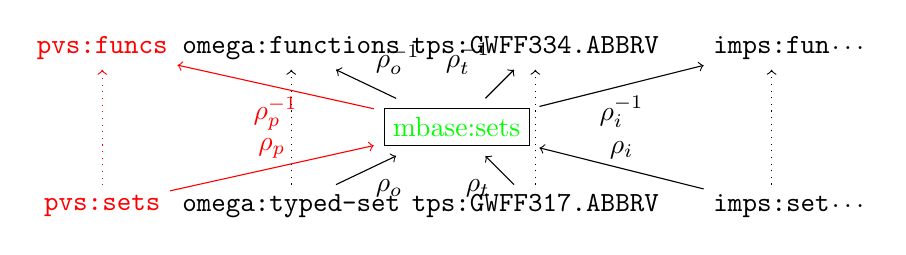
\begin{tikzpicture}
    \node (pvs) at (0,0) {\tt\color{red} pvs:sets};
    \node (omega) at (2.4,0) {\tt omega:typed-set};
    \node (tps) at (5.5,0) {\tt tps:GWFF317.ABBRV};
    \node (imps) at (8.5,0) {\tt imps:set};
    \node (etc) at (9.5,0) {\ldots};
    \node (mbase) at (4.5,1) {\fbox{\color{green} mbase:sets}};
    \draw [->,color=red] (pvs) -- node[above] {\color{red}$\rho_p$} (mbase);
    \draw[->] (omega) -- node[below right]  {$\rho_o$} (mbase);
    \draw[->] (tps) -- node[below left] {$\rho_t$} (mbase);
    \draw[->] (imps) -- node[above] {$\rho_i$} (mbase);
    \node (pvs1) at (0,2) {\tt\color{red} pvs:funcs};
    \node (omega1) at (2.4,2) {\tt omega:functions};
    \node (tps1) at (5.5,2) {\tt tps:GWFF334.ABBRV};
    \node (imps1) at (8.5,2) {\tt imps:fun};
    \node (etc1) at (9.5,2) {\ldots};
    \draw [->,color=red](mbase) -- node[below] {\color{red}$\rho_p^{-1}$} (pvs1);
    \draw[->] (mbase) -- node[above right] {$\rho_o^{-1}$} (omega1);
    \draw[->] (mbase) -- node[above left] {$\rho_t^{-1}$} (tps1);
    \draw [->] (mbase) -- node[below] {$\rho_i^{-1}$} (imps1);
    \draw[->,dotted,color=red] (pvs) -- (pvs1);
    \draw[->,dotted] (omega) -- (omega1);
    \draw[->,dotted] (tps) -- (tps1);
    \draw[->,dotted] (imps) -- (imps1);
  \end{tikzpicture}
\end{myfig}

Note that {\emph{technically}} we do not need to change the interface language of the
mathematical software systems\footnote{This is important if we want to integrate
  proprietary software systems, where we have no control over the interfaces.}, we only
rationally reconstruct their meaning in terms of the new integration theory, which can act
as a gold standard for the integration. {\emph{Socially}} the existence of the new
standard theory may prompt a migration to the nomenclature and coverage of the integration
theory. Note furthermore, that we have only treated the simple case, where the
mathematical conceptualizations underlying the software systems are already explicitly
given in a library. For many mathematical software systems the underlying
conceptualizations and assumptions are only documented in scientific papers, user manuals,
or inscribed into the code. For such systems, {\defemph{interface
    theories\twin{interface}{theory}}} that make them explicit have to be developed to
pursue the integration strategy presented above. Of course, this process needs a lot of
manual labor, but leads to true interoperability of mathematical software systems, which
can now re-use the work of others.

Finally note that the integration only works as smoothly as in our scenario, if the
systems involved make assumptions about mathematical objects that are compatible with each
other. In most cases, incompatibilities can be resolved by renaming concepts apart,
e.g. one system considers set union to be a binary operation, while the other considers it
as $n$-ary. Here, the integration theory would supply two distinct (though possibly
semantically related) concepts; The theory-based integration approach allows to explicitly
disambiguate the concepts and thus prevent confusion and translation errors. In very few
cases, systems are truly incompatible e.g. if one assumes an axiom which the other
rejects. In this case the theory based integration approach breaks down --- indeed a
meaningful integration seems impossible and unnecessary.
\end{omgroup}

\begin{omgroup}[id=logics.integrating]{A Hierarchy of Logical Languages}
  In the example above we made use of the fact that theorem proving systems are simpler to
  deal with than other mathematical software systems, since they encode the underlying
  assumptions explicitly into mathematical libraries. Unfortunately though, this is only
  partially true the underlying base logics are usually not treated in this
  way. Fortunately, logical concepts are treated in {\omdoc} just like ordinary ones: by
  content markup in {\cmathml} or {\openmath}, so that there is no fundamental barrier to
  treating them as the theory contexts above; we only have to come up with interface
  theories for them. We have done just that when we equipped various logic-based systems
  with {\omdoc} interfaces observing that even though the systems are of relatively
  different origin, their representation languages share many features:
  \begin{itemize}
  \item {\tps} and {\pvs} are based on a simply typed $\lambda$-calculus and only use type
    polymorphism in the parsing stage, whereas {\OMEGA} and {\lambdaclam} allow ML-style
    type polymorphism.
  \item {\OMEGA}, {\inka} and {\pvs} share a higher sort concept, where sorts are
    basically unary predicates that structure the typed universe.
  \item {\pvs} and {\coq} allow dependent- and record types as basic representational
    features.
  \end{itemize}
  but also differ on many others: for instance {\inka}, {\pvs}, and {\coq} explicitly
  support inductive definitions, but by very different mechanisms and on differing
  levels. {\coq} uses a constructive base logic, whereas the other systems are classical.
  The similarities are not that surprising, all of these systems come from similar
  theoretical assumptions (most notably the Automath project~\cite{Bruijn80}), and inherit
  the basic setup (typed $\lambda$-calculus) from it. The differences can be explained by
  differing intuitions in the system design and in the intended applications.

\begin{myfig}{logics-hierarchy}{A Hierarchy of Logical Languages}\vspace*{-.5cm}
  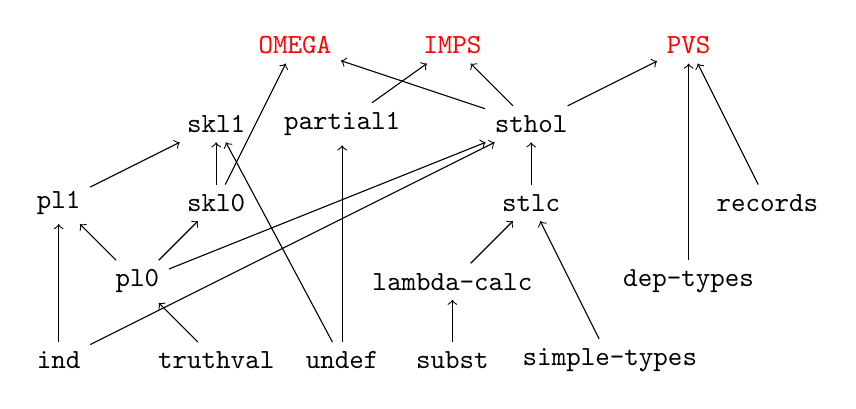
\begin{tikzpicture}
  \node (tv) at (2,0) {{\tt{truthval}}};
  \node (pl0) at (1,1) {{\tt{pl0}}};
  \node (skl0) at (2,2) {{\tt{skl0}}};
  \node (ind) at (0,0) {{\tt{ind}}};
  \node (pl1) at (0,2) {{\tt{pl1}}};
  \node (undef) at (3.6,0) {{\tt{undef}}};
  \node (skl1) at (2,3) {{\tt{skl1}}};
  \node (partial1) at (3.6,3) {{\tt{partial1}}};
  \node (subst) at (5,0) {{\tt{subst}}};
  \node (lambda-calc) at (5,1) {{\tt{lambda-calc}}};
  \node (stypes) at (7,0) {{\tt{simple-types}}};
  \node (dtypes) at (8,1) {{\tt{dep-types}}};
  \node (stlc) at (6,2) {{\tt{stlc}}};
  \node (sthol) at (6,3) {{\tt{sthol}}};
  \node (records) at (9,2) {{\tt{records}}};
  \node (imps) at (5,4) {{\tt{\color{red} IMPS}}};
  \node (pvs) at (8,4) {{\tt{\color{red} PVS}}};
  \node (omega) at (3,4) {{\tt{\color{red} OMEGA}}};

  \draw[->] (tv) -- (pl0);
  \draw[->] (pl0) -- (pl1);
  \draw[->] (pl0) -- (skl0);
  \draw[->] (ind) -- (pl1);
  \draw[->] (pl1) -- (skl1);
  \draw[->] (skl0) -- (skl1);
  \draw[->] (undef) -- (skl1);
  \draw[->] (undef) -- (partial1);
  \draw[->] (subst) -- (lambda-calc);
  \draw[->] (lambda-calc) -- (stlc);
  \draw[->] (stypes) -- (stlc);
  \draw[->] (stlc) -- (sthol);
  \draw[->] (pl0) -- (sthol);
  \draw[->] (ind) -- (sthol);
  \draw[->] (partial1) -- (imps);
  \draw[->] (sthol) -- (imps);
  \draw[->] (dtypes) -- (pvs);
  \draw[->] (records) -- (pvs);
  \draw[->] (sthol) -- (pvs);
  \draw[->] (sthol) -- (omega);
  \draw[->] (skl0) -- (omega);
\end{tikzpicture}
\end{myfig}
We have started to provide a standardized, well-documented set of content dictionaries for
logical languages in the {\omdoc} distribution. These are organized hierarchically, as
depicted in {\myfigref{logics-hierarchy}}.  In essence, the structured theory mechanism in
{\omdoc} is used to create a language hierarchy that inter-relates the various
representation formats of existing theorem provers. For instance the simply typed
$\lambda$-calculus can be factored out (and thus shared) of the representation languages
of all theorem proving systems above. This makes the exchange of logical formulae
via the {\omdoc} format very simple, if they happen to be in a suitable common fragment:
In this case, the common ({\openmath}/{\omdoc}) syntax is sufficient for communication.
\end{omgroup}

\begin{omgroup}[id=logic.morphisms]{Logic Interoperability via Logic Morphisms}
  In theoretical accounts of the integration of logical languages, one finds categorical
  accounts like the one described in {\sref{hets}} or {\indextoo{proof-theoretic}}
  ones based on definitions like the one below. Both mesh well with the {\omdoc}
  representation format and its theory level; we will show this for the proof-theoretic
  account here.

\begin{definition}[id=logical-system.def]
  A {\defemph{logical system}} $\cS=(\cL,\cC)$ consists of a language $\cL$ (i.e. a set of
  well-formed formulae) and a calculus $\cC$ (i.e. a set of inference rules).  A calculus
  gives us a notion of a $\cC$-derivation of $\bA$ from $\cH$, which we will denote by
  $\cD\colon\cH\vdash_\cC\bA$. Let $\cS$ and $\cS'$ be logical systems, then a
  {\defemph{logic morphism}} $\cF\colon\cS\to\cS'$ consists of a {\defemph{language
      morphism}} $\cF^\cL\colon\cL\to\cL'$ and a {\defemph{calculus morphism}} $\cF^\cD$
  from $\cC$-derivations to $\cC'$-derivations, such that for any $\cC$-derivation
  $\cD\colon\cH\vdash_\cC\bA$ we have $\cF^\cD(\cD)\colon
  \cF^\cL(\cH)\vdash_{\cC'}\cF^\cL(\bA)$.
\end{definition}
\def\sortn{{\mathbb N}}\def\sortb{{\mathbb B}}\def\sorta{{\mathbb A}} \def\sortc{{\mathbb
    C}}\def\ofsort{\colon} The intuition behind this is that logic morphisms transport
proofs between logical systems. Logic morphisms come in all shapes and sizes, a well-known
one is the relativization morphism from sorted logics to unsorted ones, for instance the
morphism $\cR$ from sorted first-order logic (${\mathbb S} FOL$) to unsorted first-order
logic ($FOL$). For every sorted constant $\cR$ introduces an axiom
e.g. $\cR([+\colon\sortn\rightarrow\sortn\rightarrow\sortn])= \forall
X,Y\sdot\sortn(X)\land\sortn(Y)\implies\sortn(X+Y)$. On formulae sorted quantifications
are translated into unsorted ones guarded by sort predicates, e.g.  $\cR(\forall
X_\sortb\sdot\bA)=\forall X\sdot\sortb(X)\implies\cR(\bA)$. Finally, for proofs we have
the correspondence given in {\myfigref{Relativization}}, where $\sorta,\sortb,\ldots$ are
sort symbols.
\begin{myfig}{Relativization}{Relativization Morphism on Proofs}\vspace*{-.5cm}
  \begin{textnd}
    \setbox0=\hbox{\ibnc{\bA\ofsort\sortb\rightarrow\sortc}
                        {\bB\ofsort\sortb}
                        {\bA\bB\ofsort\sortc}
                        {}}
    \setbox1=\hbox{\ibnc{\ianc{\forall X\sdot\sortb(X)\implies\sortc(\bA X)}
                              {\sortb(\bB)\implies\sortc(\bA\bB)}
                              {}}
                        {\sortb(\bB)}
                        {\sortc(\bA\bB)}
                        {}}
    \cR\left(\raisebox{-.3cm}{\box0}\vspace*{-.5cm}\right)
    \;\;=\;\;\raisebox{-.8cm}{\box1}\\
    \setbox0=\hbox{\ibnc{\forall X_\sortb\sdot\bA}
                        {\bB\colon\sortb}
                        {[\bB/X]\bA}
                        {}}
    \setbox1=\hbox{\ibnc{\ianc{\forall X\sdot\sortb(X)\implies\cR(\bA)}
                              {\sortb(\cR(\bB))\implies\cR([\bB/X]\bA)}
                              {}}
                        {\sortb(\bB)}
                        {\cR([\bB/X]\bA)}
                        {}}
    \cR\left(\raisebox{-.3cm}{\box0}\vspace*{-.5cm}\right)
    \;\;=\;\;\raisebox{-.8cm}{\box1}
  \end{textnd}
\end{myfig}

In Definition~\ref{def:logical-system} a logical system is a two-partite object consisting
of a language and a calculus. In the {\twintoo{ontologically}{promiscuous}} {\omdoc}
format both parts are represented largely like ordinary mathematically concepts. The
notable exception is that proofs have a slightly dual representation, but inference rules
of a calculus are still represented as symbols via the
{\twintoo{Curry-Howard}{isomorphism}} (see {\extref{spec}{proofs}}). Thus a logical system
can be represented as an {\omdoc} theory as we did above, moreover, the
{\twintoo{logic}{morphism}} $\cR$ can simply be encoded as a theory inclusion from
${\mathbb S} FOL$ to $FOL$ mapping ${\mathbb S} FOL$ constants for inference rules to
$FOL$ terms for proofs. The condition on the form of derivations in
Definition~\ref{def:logical-system} now simply takes on the form of a type compatibility
condition.
\end{omgroup}
\end{omgroup}
%%% Local Variables: 
%%% mode: latex
%%% TeX-master: "../main"
%%% End: 

% LocalWords:  rpc pvs emptyset superset fullset setminus exclunion mbase tps
% LocalWords:  Automath tv truthval skl undef subst calc stypes dtypes dep stlc
% LocalWords:  sthol zf ZF RZF koh Koh ohori bmv mv izf iZF isorts irecords
% LocalWords:  hets
